\documentclass{beamer}
\usetheme{Madrid}
\usepackage{lmodern}% http://ctan.org/pkg/lm
\setbeamersize{text margin left = 2.5em}
\setbeamersize{text margin right = 2.5em}
\usepackage{color}
\usepackage{graphicx}
\usepackage{MnSymbol}
\usepackage{amsmath}
\usepackage{comment}
\usepackage{tikz}
\usepackage{subfigure}
\usepackage{listings}
\usetikzlibrary{automata}

%\usepackage[backend=bibtex,sorting=none]{biblatex}
%\addbibresource{E:/Papers/LiuLab} %BibTeX�����ļ���λ��
%\setbeamerfont{footnote}{size=\tiny}
\setbeamertemplate{theorems}[numbered]
\setbeamertemplate{caption}[numbered]
%% ʹ�ý�ע���õ�Ƭijҳ���Ӳο����ס�
%% ��������ʹ�ã�\footfullcite{bib_item} %����item
%% \usepackage{anyfontsize}%% allowing font sizes at arbitrary sizes
\logo{
\includegraphics[height=0.05\textwidth]{Pic/logo}}
\newtheorem{df}{Definition}
\newtheorem{DF}{DEFINITION}
\newtheorem{prop}{Proposition}
\newtheorem{thm}{Theorem}
\newtheorem{cor}{COROLLARY}
\newtheorem{lm}{LEMMA}
% ----------------------------------------------------------------------------------------
% TITLE PAGE
% ----------------------------------------------------------------------------------------

\title{P02 CSP (GAC)}
% The short title appears at the bottom of every slide, the full title is only on the title page

\author{Suixin Ou} % Your name
\institute[SYSU] % Your institution as it will appear on the bottom of every slide, may be shorthand to save space
{
  School of Computer Science\\
  Sun Yat-sen University \\ % Your institution for the title page
  \medskip
  % Your email address
}

\date{October 19, 2021} % Date, can be changed to a custom date

\AtBeginSection[]
{
  \begin{frame}
    \tableofcontents[currentsection,currentsubsection]
  \end{frame}
}

\begin{document}

\begin{frame}
  \titlepage
\end{frame}

\begin{frame}
  \frametitle{Task}
  \begin{block}{Problem}
\begin{itemize}
    \item Futoshiki is a board-based puzzle game. It is playable on a square board having a given fixed size.

     \item The purpose of the game is to discover the digits hidden inside the board’s cells; each cell is filled with a digit between 1 and the board’s size. On each row and column each digit appears exactly once; therefore, when revealed, the digits of the board form a so-called Latin square.

   \item  At the beginning of the game some digits might be revealed. The board might also contain some inequalities between the board cells; these inequalities must be respected and can be used as clues in order to discover the remaining hidden digits.

   \item  Each puzzle is guaranteed to have a solution and only one.

    \item You can play this game online: http://www.futoshiki.org/.
    \end{itemize}
  \end{block}
\end{frame}





\begin{frame}
  \frametitle{Task}
  \begin{block}{Input-output}
    \begin{itemize}
      \item Input: a n x n matrix of initial state, and a list of inequal constraints.


	  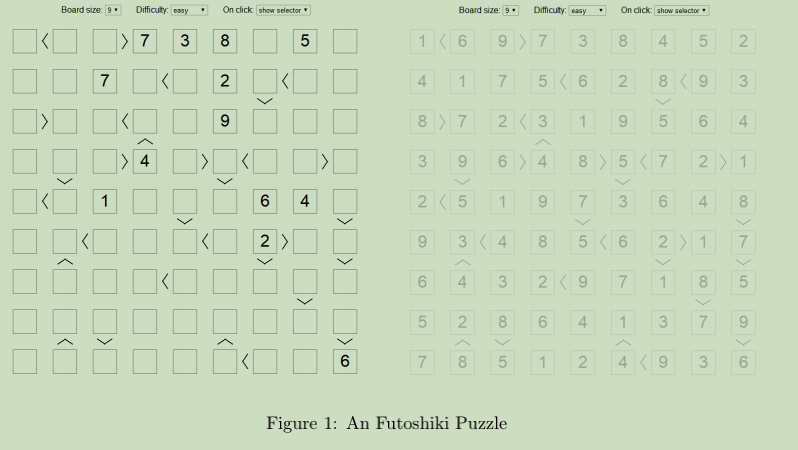
\includegraphics[width=0.7\textwidth]{Pic/figure1}

      \item Output: the n x n matrix of the terminate state that satisfys all constraints (including inequal constraints, row and column constraints).
    \end{itemize}
  \end{block}
\end{frame}
\begin{frame}

  \frametitle{Task}

  \begin{block}{Grading}
    \begin{itemize}
      \item Describe with sentences the main ideas of the GAC algorithm and the main differences between the GAC and the forward checking (FC) algorithm. (10 points)
\item %When enforcing GAC on constraint $C$, if for a variable $V$ in the scope of $C$, we remove a value $d$ from CurDom[V], why do we need to check again for the consistency of any constraint containing $V$ in its scope? Some student suggests that we do not need to check again for the consistency of $C$. Is this correct, and why?

     The GAC$\_$Enforce procedure from class acts as follows: when removing d from CurDom[V], push all constraints $C'$ such that $V\in scope(C')$ and $C'\not\in$ GACQueue onto GACQueue. What's the reason behind this operation? Can it be improved and how? (20 points)

\item Use the GAC algorithm to implement a Futoshiki solver by \textbf{C++} or \textbf{Python}. (20 points)
\item Explain any ideas you use to speed up the implementation. (10 points)
\item Run the following 5 test cases to verify your solver's \textbf{correctness}. (20 points)

    \end{itemize}
  \end{block}
\end{frame}


\begin{frame}    \frametitle{Task}

  \begin{block}{Grading}
    \begin{itemize}
\item Run the FC algorithm you implemented in E04 and the GAC algorithm you implemented in Task 3 on the 5 test cases, \textbf{fill in the following table and analyse the reasons behind the experimental results}. In the table,
    ``Total Time" means the total time the algorithm uses to solve the test case,  ``Number of Nodes Searched" means the total number of nodes traversed by the algorithm, 
    and ``Average Inference Time Per Node" means the average time for constraint propagation (inference) 
used in each node (note that this time is not equal to the total time divided by the number of nodes searched). (20 points)

    \end{itemize}
  \end{block}

\end{frame}





\begin{frame}    \frametitle{Task}

    \begin{figure}[htbp]
    \centering
    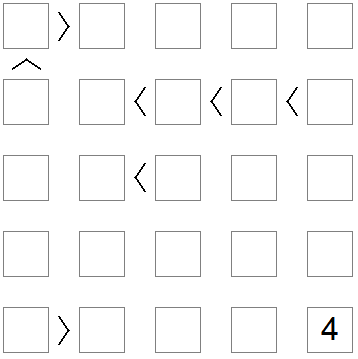
\includegraphics[width=4.5cm]{Pic/f1}
    \qquad
    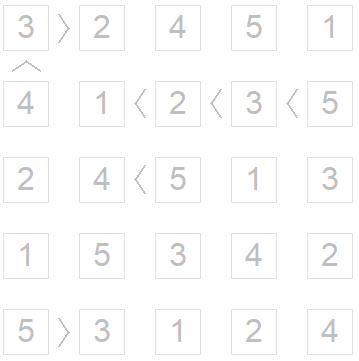
\includegraphics[width=4.5cm]{Pic/f1s}
    \caption{Futoshiki Test Case 1}
    \label{fig:case11}
  \end{figure}
\end{frame}
\begin{frame}    \frametitle{Task}
        \begin{figure}[htbp]
    \centering
    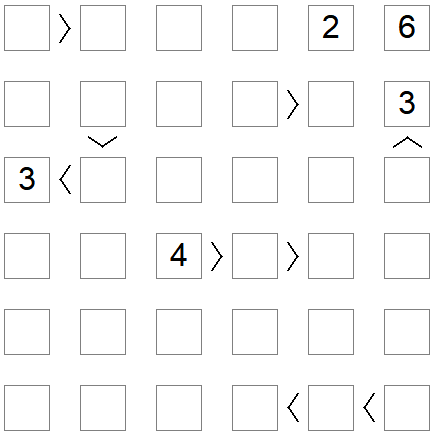
\includegraphics[width=4.5cm]{Pic/f2}
    \qquad
    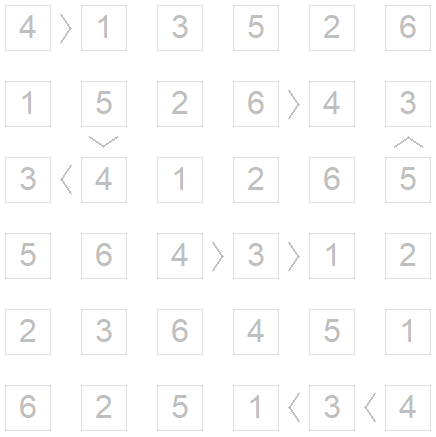
\includegraphics[width=4.5cm]{Pic/f2s}
    \caption{Futoshiki Test Case 2}
    \label{fig:case22}
  \end{figure}
\end{frame}
\begin{frame}    \frametitle{Task}
        \begin{figure}[htbp]
    \centering
    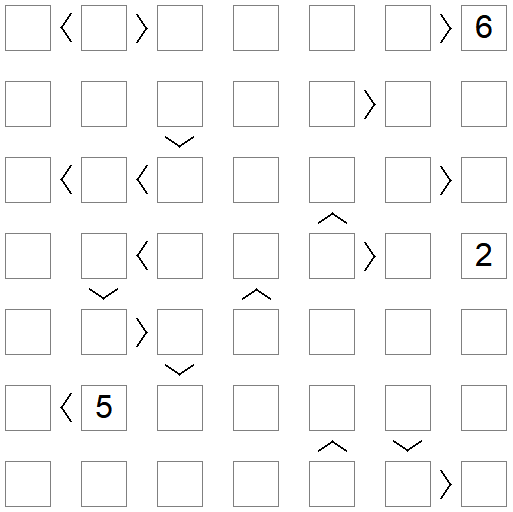
\includegraphics[width=4.5cm]{Pic/f3}
    \qquad
    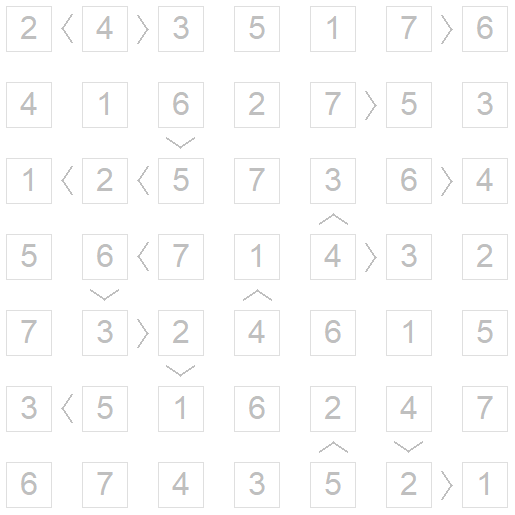
\includegraphics[width=4.5cm]{Pic/f3s}
    \caption{Futoshiki Test Case 3}
    \label{fig:case33}
  \end{figure}
\end{frame}
\begin{frame}    \frametitle{Task}
        \begin{figure}[htbp]
    \centering
    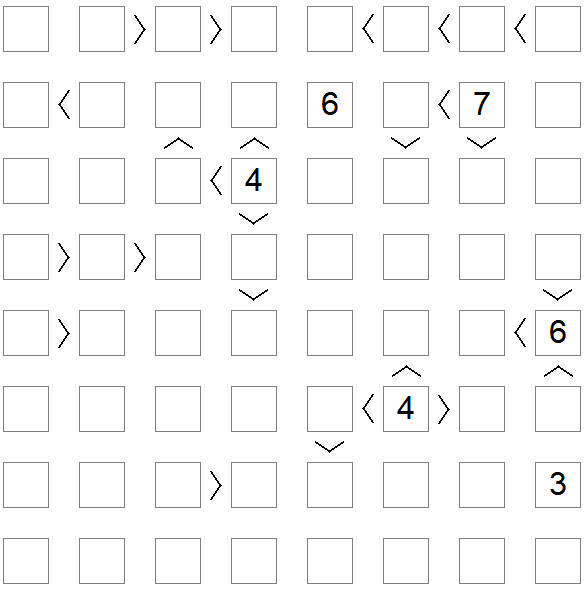
\includegraphics[width=4.5cm]{Pic/f4}
    \qquad
    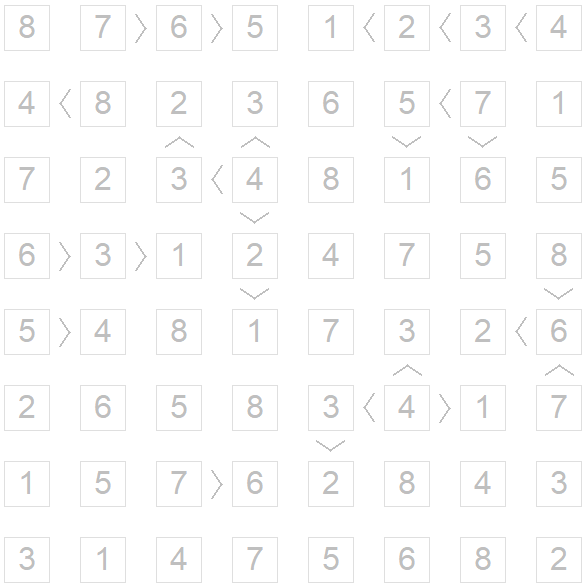
\includegraphics[width=4.5cm]{Pic/f4s}
    \caption{Futoshiki Test Case 4}
    \label{fig:case44}
  \end{figure}
\end{frame}
\begin{frame}    \frametitle{Task}
        \begin{figure}[htbp]
    \centering
    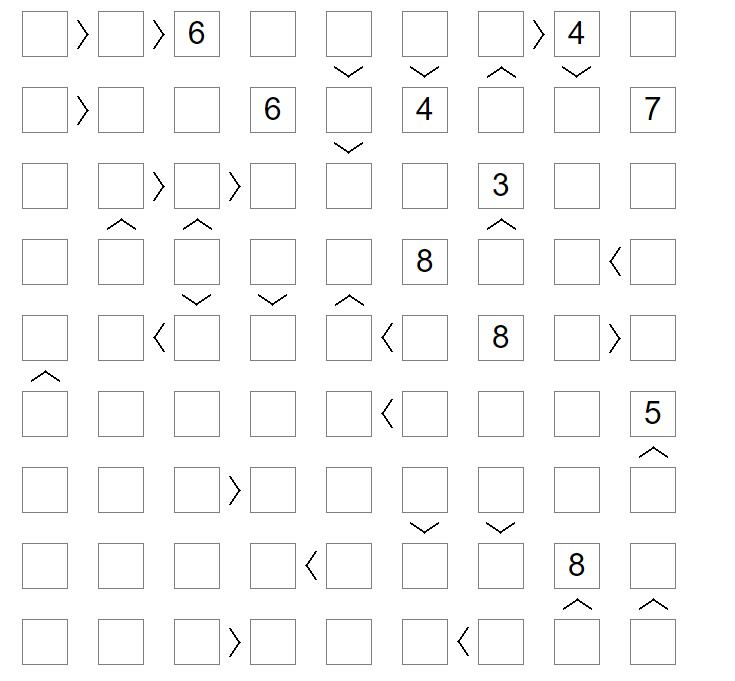
\includegraphics[width=4.5cm]{Pic/f5}
    \qquad
    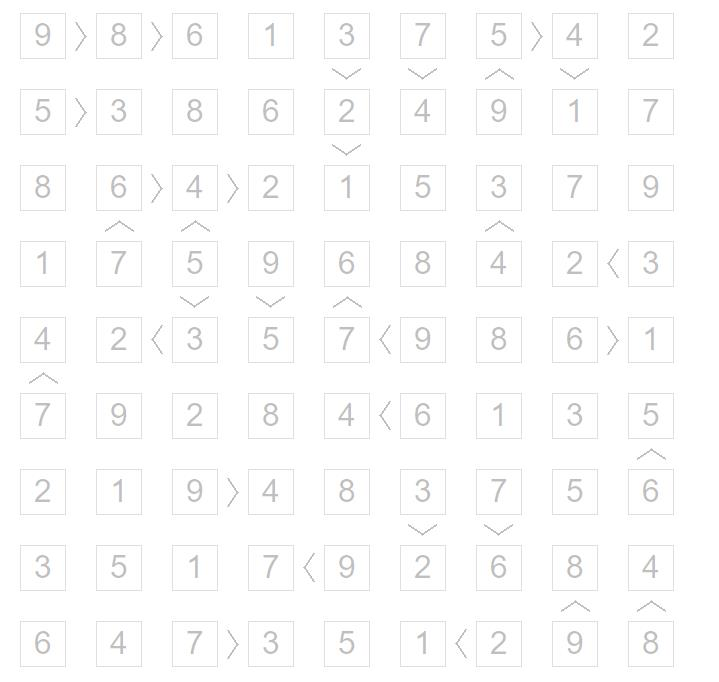
\includegraphics[width=4.5cm]{Pic/f5s}
    \caption{Futoshiki Test Case 5}
    \label{fig:case55}
  \end{figure}

\end{frame}

\begin{frame}    \frametitle{Task}

 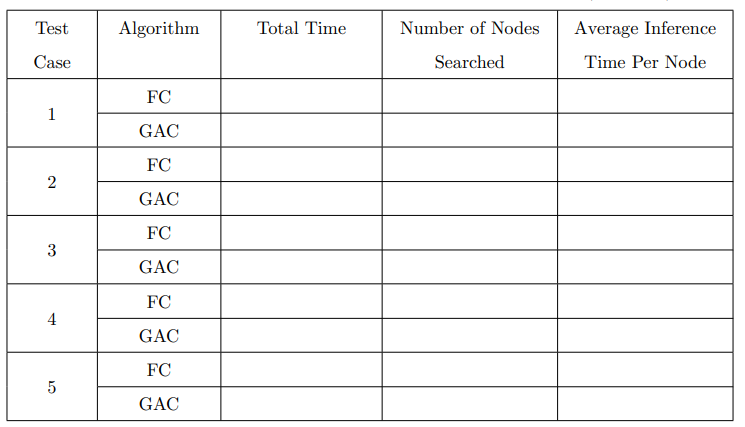
\includegraphics[width=1.0\textwidth]{Pic/tab}


\end{frame}

\begin{frame} \frametitle{Task}
  \begin{block}{Submission}
    pack your report \texttt{P02\_YourNumber.pdf} and source code into zip file \texttt{P02\_YourNumber.zip}, then send it to \texttt{ai\_course2021@163.com}.
  \end{block}
\end{frame}

\begin{frame} 
  \frametitle{Solution}
  Algorithm procedure
  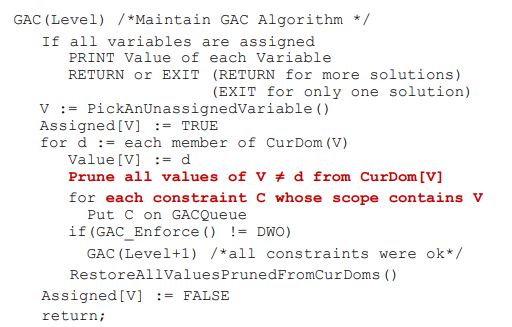
\includegraphics[width=0.8\textwidth]{Pic/gac1}
\end{frame}

\begin{frame}
  \frametitle{Solution}
  Algorithm procedure
  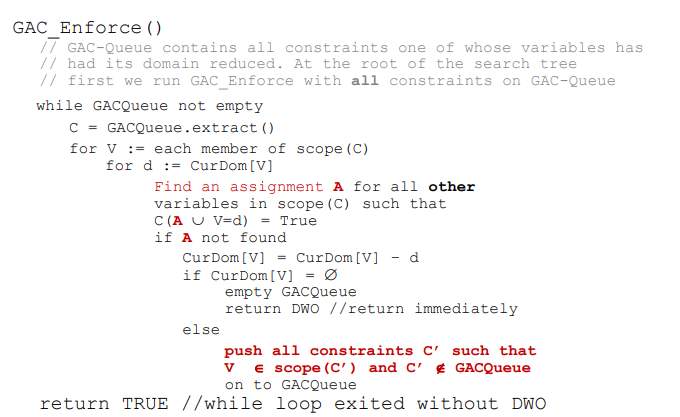
\includegraphics[width=0.8\textwidth]{Pic/gac2}
\end{frame}


\begin{frame}
  \frametitle{Solution}
  \begin{columns}
    \begin{column}{.5\linewidth}
      Read input
      
      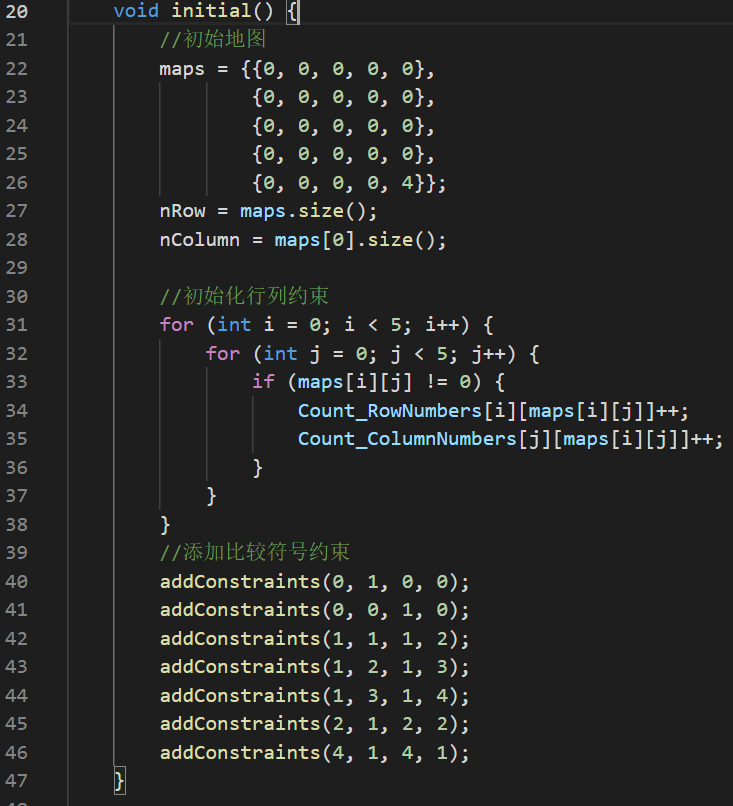
\includegraphics[width=1.0\textwidth]{Pic/ini}

      
      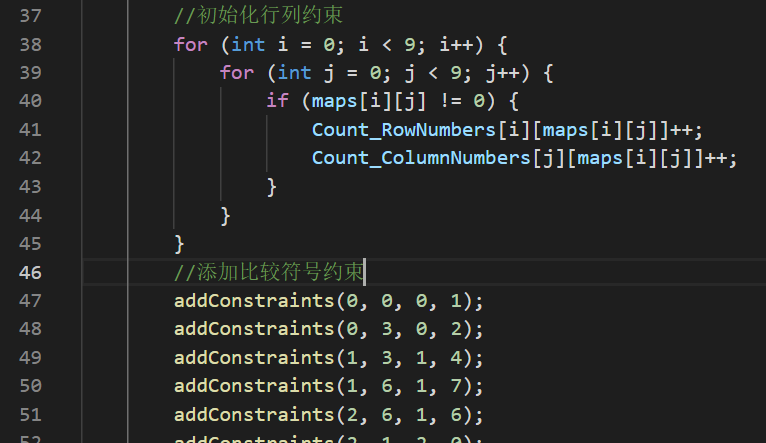
\includegraphics[width=1.0\textwidth]{Pic/addC}
    \end{column}
    \begin{column}{.5\linewidth}
      Visualize output
      
      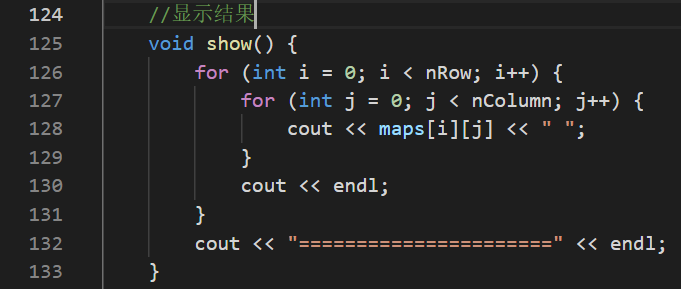
\includegraphics[width=1.05\textwidth]{Pic/print}
    \end{column}
  \end{columns}

\end{frame}

\begin{frame}
  \frametitle{Solution}
      Check whether conditions are all satisfied.
      \textbf{You should finish a check function for the Generalized Arc Consistency(GAC) algorithm.}
      
      
      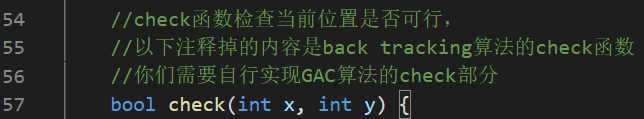
\includegraphics[width=.9\textwidth]{Pic/check}
      Search for correct solution.
      
      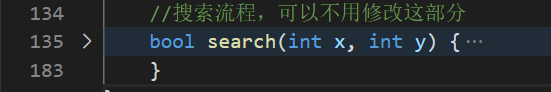
\includegraphics[width=.9\textwidth]{Pic/search}

\end{frame}



%-----------------------------------------------------------------------------------------

\begin{frame}
  \Huge{\centerline{The End}}
\end{frame}

% ----------------------------------------------------------------------------------------


\end{document}
